% Group Number 31 -- Human or AI? Kaggle report (course template, filled in).
% Self-contained: upload only this file to Overleaf. Blocks between "% <<gen ..." and "% gen>>" are copied from
% the repository's generated results by reports/inline_tables.py; do not edit them by hand.
\documentclass[11pt,letterpaper]{article}
\usepackage[margin=0.86in]{geometry}
\usepackage[T1]{fontenc}
\usepackage[utf8]{inputenc}
\usepackage{lmodern}
\usepackage{xcolor}
\usepackage{tabularx,booktabs,array,longtable}
\usepackage{enumitem}
\usepackage{hyperref}
\usepackage{fancyhdr}
\usepackage{lastpage}
\usepackage{titlesec}
\usepackage{amsmath,amssymb}
\usepackage{microtype}
\usepackage{needspace}
\usepackage{ragged2e}
\usepackage{pgfplots}
\pgfplotsset{compat=1.18}
\definecolor{navy}{HTML}{19334C}
\definecolor{teal}{HTML}{236B82}
\definecolor{soft}{HTML}{EFF5F7}
\definecolor{muted}{HTML}{52616B}
\definecolor{copper}{HTML}{C0763A}
\hypersetup{colorlinks=true,linkcolor=teal,urlcolor=teal,citecolor=teal}
\titleformat{\section}{\Large\bfseries\color{navy}}{\thesection.}{0.6em}{}
\titleformat{\subsection}{\large\bfseries\color{navy}}{\thesubsection}{0.6em}{}
\titleformat{\subsubsection}{\normalsize\bfseries\color{navy}}{\thesubsubsection}{0.6em}{}
\titlespacing*{\section}{0pt}{15pt}{6pt}
\titlespacing*{\subsection}{0pt}{10pt}{4pt}
\setlength{\parindent}{0pt}
\setlength{\parskip}{4.5pt}
\setlength{\headheight}{15pt}
\renewcommand{\arraystretch}{1.16}
\setlist[itemize]{topsep=3pt,itemsep=2pt,leftmargin=1.4em}
\setlist[enumerate]{topsep=3pt,itemsep=2pt,leftmargin=1.5em}
\pagestyle{fancy}
\fancyhf{}
\fancyhead[L]{\small\color{muted} Applied Machine Learning \textbar{} Cornell Tech}
\fancyhead[R]{\small\color{muted} Human or AI?}
\fancyfoot[C]{\small\color{muted} Page \thepage\ of \pageref{LastPage}}
\renewcommand{\headrulewidth}{0.3pt}
\newcommand{\placeholder}[1]{\par\noindent\textcolor{teal}{\textit{[Your response: #1]}}\par\vspace{0.3em}}
\newcommand{\figplaceholder}[1]{\par\noindent\fcolorbox{teal}{soft}{\parbox[c][1.15in][c]{0.94\linewidth}{\centering\textcolor{muted}{Insert #1 here}}}\par}
\newcommand{\question}[2]{\needspace{4\baselineskip}\par\addvspace{0.45em}\noindent\textbf{#1}\quad #2\par\nobreak\vspace{0.1em}}
\newcommand{\smallnote}[1]{{\small\color{muted}#1}}
\newcolumntype{Y}{>{\RaggedRight\arraybackslash}X}
\newcommand{\commit}[2]{\href{https://github.com/ZhenmanShen/human-or-ai-submissions/commit/#1}{\texttt{#2}}}
\expandafter\def\expandafter\UrlBreaks\expandafter{\UrlBreaks\do\-\do\.}
\newcommand{\hf}[1]{{\small\nolinkurl{#1}}}% Hugging Face ids; may break at / - .
\begin{document}
\thispagestyle{empty}
\vspace*{0.2in}
{\color{teal}\bfseries CORNELL TECH \textbar{} APPLIED MACHINE LEARNING}\par
\vspace{0.15in}
{\Huge\bfseries\color{navy} Human or AI?}\par
\vspace{0.07in}
{\LARGE\color{navy} Kaggle Competition Report --- Group Number 31}\par
\vspace{0.17in}

\textbf{Report Template: }\href{https://www.overleaf.com/project/6ae1fc85355dcf680137d898/share#f2777b20d3adeeecfac9096f78008e2f8daa0ff4be43de3b}{TEMPLATE}

\textbf{Github Repository Template: }\href{https://github.com/sekhari/human-or-ai-submissions}{REPO}

\textbf{Welcome to the competition!} Your task is to build a machine learning classifier that predicts whether a passage was written by a human or generated by an AI model. You will use a labeled training set, an additional unlabeled set, and a held-out Kaggle test set. The aim is not just a high leaderboard score: we want you to compare methods, design careful experiments, understand generalization, and explain what your results actually show.

You are encouraged to try several approaches. A well-tested logistic regression or support vector machine is just as legitimate as a neural network. The project is designed to be approachable on a laptop; a GPU is \emph{not required} for full credit.

\vspace{0.06in}
\begin{tabularx}{\linewidth}{@{}>{\bfseries}p{1.58in}Y@{}}
Team / members & Zhenman Shen (zs476), Giorgi Samushia (gs799), Aynan Kareem (ak2896) \\
Kaggle team name & Group Number 31 \\
GitHub PR URL & [TODO: PR URL] \\
\end{tabularx}
\vspace{0.06in}
\subsection*{Your data}
\begin{tabularx}{\linewidth}{@{}lrrY@{}}
\toprule
\textbf{File} & \textbf{Rows} & \textbf{Labels} & \textbf{Purpose} \\
\midrule
\texttt{train.csv} & 10,000 & Visible & Supervised model development: 5,000 human (0), 5,000 AI (1) \\
\texttt{unlabeled.csv} & 3,000 & Hidden & Optional input for semi-supervised methods; required experiment \\
\texttt{test.csv} & 3,000 & Hidden & Predict the probability of AI authorship for Kaggle \\
\texttt{train\_starter\_2000.csv} & 2,000 & Visible & Convenient subset of \texttt{train.csv} for quick experiments \\
\bottomrule
\end{tabularx}

\smallnote{The starter data is a subset, not 2,000 additional labeled examples. Passages are approximately 75--350 words, with mean length near 210 words.}

\subsection*{How the test set works}
The test set mixes familiar and unfamiliar writing domains and AI generators, and includes some adversarially modified AI-written passages. You will \emph{not} receive labels, source model names, domain labels, or difficulty memberships for individual test examples. Submit a probability in $[0,1]$ for each test ID, where 1 means AI-generated. Kaggle evaluates submissions using \textbf{area under the ROC curve (AUROC)}. The \textbf{public leaderboard} covers 900 examples (30\%); the \textbf{private leaderboard} covers 2,100 (70\%) and determines the final competition performance score.


\vfill
\newpage
\section{Competition rubric and submission instructions}
\begin{tabularx}{\linewidth}{@{}Y>{\raggedleft\arraybackslash}p{0.85in}@{}}
\toprule \textbf{Component} & \textbf{Points}\\ \midrule
Kaggle private leaderboard performance & 25 \\
Model comparison and selection & 15 \\
Effect of training data size & 10 \\
Learning from unlabeled data & 5 \\
Generalization and error analysis & 20 \\
Open-ended improvements and insights & 15 \\
Code submission and GitHub PR history & 10 \\
\midrule \textbf{Total} & \textbf{100} \\ \bottomrule
\end{tabularx}

\textbf{How to use this document.} Complete the response fields and tables below; insert plots where requested. Keep your answers concise, specific, and supported by actual experiments. Points appear in brackets beside each question; no separate writing-quality grade is assigned.

\textbf{How credit is awarded.} We grade the \emph{quality of the experimental method, evidence, and interpretation}, not whether a proposed idea succeeds. \textbf{Negative results can also earn full credit} when the comparison is valid, the results are reported accurately, and the conclusions are thoughtful. For each question, make clear what you tried, what you measured, and what you learned. Do not invent scores or results.

\textbf{Submit three items:} (1) final Kaggle submission; (2) this completed report as PDF; (3) one GitHub PR link in the course repository, with runnable code, instructions and meaningful commit history. Include the PR link on the title page. Confirm upload locations and deadline time on the course site. The template for the repository is \href{https://github.com/sekhari/human-or-ai-submissions}{here}

\textbf{Compute and models.} Use models and pipelines that you can run and reproduce. Laptop-friendly training is strongly recommended; use of more expensive methods is allowed but not required for full credit. Do not use external LLM APIs to directly label or predict the competition test passages. Use only the supplied labeled dataset for supervised labels; allowed pretrained weights and AI-assisted development should be disclosed.

\textbf{Validation.} For the required controlled experiments, reserve a fixed stratified \textbf{2,000-row validation set} from \texttt{train.csv}, leaving up to 8,000 rows for training. Use the \emph{same} held-out validation set for comparisons and do not tune on test labels. You may retrain your final Kaggle model on all 10,000 labeled examples after selecting your approach. Where possible, document seeds and avoid source/near-duplicate leakage.

\textbf{Kaggle grading (25 points).} Final performance will use the private AUROC, not leaderboard rank. The intended continuous rule is $25\,\mathrm{clip}((A-0.50)/(T-0.50),0,1)$, where $A$ is your private AUROC and $T$ is the announced full-credit threshold. A provisional value of $T=0.90$ is under consideration; the instructors will confirm the fixed threshold before launch. A reference word TF-IDF and logistic regression baseline achieves approximately 0.868 private AUROC.

\textbf{Our validation protocol (used for every number below).} One fixed stratified 2,000-row validation split of \texttt{train.csv} (1,000 human, 1,000 AI; seed 20261023; ids committed in \texttt{common/val\_ids.csv}). Every model trains on the other 8,000 rows; hyperparameters are chosen by 5-fold cross-validation inside those 8,000 rows only. Kaggle files are refit on all 10,000 rows.

\section{Team information and model summary}
\question{Q0.1 [0 points].}{List team members and their main contributions.}
\begin{itemize}
\item \textbf{Zhenman Shen (zs476).} Designed the overall approach: the two-track structure, the model architectures, the candidate models and the analyses to run. Read and inspected the data and adjusted the pipelines to what it showed. Compared local against Kaggle scores, diagnosed the classical models' drop and directed their fix. Ran the Kaggle submissions and the repository.
\item \textbf{Giorgi Samushia (gs799).} Classical (from-scratch) track: reviewed the TF-IDF, stylometric and Transformer models and their hyperparameter searches, and the data-size and unlabeled-data experiments (Q2--Q3).
\item \textbf{Aynan Kareem (ak2896).} Pretrained track and evaluation: reviewed the LM-feature and fine-tuned models, the subgroup and error analysis, and the out-of-distribution results (Q4--Q5).
\end{itemize}
All three members reviewed the report. Code was written and run with Claude Code under our direction (Q6.3).

\question{Q0.2 [0 points].}{Summarize your final approach in 3--5 sentences. What is the overall pipeline from raw text to probability?}
Our final submission, \textbf{blend A}, scores each raw passage with seven models. Four are LightGBM \cite{lightgbm} heads on statistics of frozen pretrained language models: GPT-2 and GPT-2-medium token log-probabilities, ranks and entropies \cite{gpt2}, and Binoculars scores from Qwen2.5-0.5B/1.5B \cite{binoculars,qwen25}, plus 43 style features. Three are fine-tuned encoders: RoBERTa-base \cite{roberta}, DeBERTa-v3-large \cite{debertav3} and the RoBERTa-large GPT-2-output detector \cite{solaiman2019}. Each model's score is mapped to a percentile of its own out-of-fold training scores, and the probability is the weighted mean of these percentiles (weights 3, 3, 2, 1, 1, 1, 1). The weights were chosen on a held-out out-of-distribution proxy, because validation could not separate the candidates. Our best fully from-scratch model, a TF-IDF logistic regression on raw-character and topic-free n-grams, reaches 0.96374 public AUROC.

\question{Q0.3 [0 points].}{Record your final scores (enter private score only once it is revealed).}
\begin{tabularx}{\linewidth}{@{}Yp{1.8in}@{}}\toprule Metric & Your score \\ \midrule Validation AUROC (blend A, fixed 2,000 rows) & 0.99990 \\ Kaggle public AUROC (blend A) & 0.99161 \\ Kaggle private AUROC & [TODO: after reveal] \\ \bottomrule\end{tabularx}

\newpage
\section{Model comparison and selection (15 points)}
\textbf{Learning goal:} demonstrate sensible representation choices, comparisons of at least three approaches, appropriate hyperparameter selection, and evidence-based selection of the final classifier.

\question{Q1.1 [3 points].}{How did you preprocess and represent the text? Specify tokenization, normalization, word/character features or embeddings, and any feature extraction choices. Why?}
We keep case, spacing, line breaks and Unicode, because formatting is signal here: removing it lowered every feature-based model on held-out shifted text (Q5). We built two tracks.
\begin{itemize}
\item \textbf{From scratch (no pretrained weights).}
  \begin{itemize}
  \item \textbf{C1} stacks three sublinear TF-IDF views \cite{sklearn}: word 1--2-grams, raw-text character 1--5-grams (layout visible), and word 1--3-grams over \emph{text-distorted} input \cite{stamatatos2017}. Distortion masks every word outside the 300 most frequent training words, so topic is removed and style is kept.
  \item \textbf{C2} computes 101 stylometric measurements \cite{ma2023}: burstiness, type--token ratio, punctuation and function-word rates, readability, line and blank-line structure, homoglyph counts.
  \item \textbf{C3} joins single line breaks (blank lines kept), distorts the text, and trains a 12k byte-level BPE \cite{bpe} on train plus \texttt{unlabeled.csv} for a small Transformer \cite{transformer}.
  \end{itemize}
\item \textbf{Pretrained.} Frozen LMs summarise how predictable each token is, which transfers across topics. Encoders are fine-tuned on sub-word tokens. The checkpoints in our blends are listed in Table~\ref{tab:pretrained} (Appendix A).
\end{itemize}
All vocabularies and word lists are fit on training rows only.

\question{Q1.2 [5 points].}{Which \textbf{three or more} modeling approaches did you try? Keep the labeled validation partition fixed across models.}
The six models we submitted to Kaggle, all trained on the same 8,000 rows and scored on the same 2,000:

{\small\begin{tabularx}{\linewidth}{@{}>{\RaggedRight}p{0.95in}Yrrrr@{}}\toprule
Model & Text representation & Train AUROC & Val. AUROC & Train time & Kaggle public \\ \midrule
% <<gen file:common/tables/six_models_q12.tex
Blend A & 7-model CDF blend: 3 frozen-LM + style heads, GPT-2 stats-only head, 3 fine-tuned encoders; weights 3,3,2,1,1,1,1 & 1.00000 & 0.99990 & 53.6 min & 0.99161 \\
Blend B & 4 frozen-LM token-statistics + style heads (GPT-2, GPT-2-medium, 2 Qwen2.5 Binoculars), equal weights & 1.00000 & 0.99985 & 16 s & 0.98848 \\
Blend C & blend B + fine-tuned RoBERTa-base, equal weights & 1.00000 & 0.99987 & 4.3 min & 0.98845 \\
\midrule
C1 TF-IDF + LR & word 1--2 + raw char 1--5 + distorted-text word 1--3 TF-IDF $\to$ logistic regression & 1.00000 & 0.99678 & 23 s & 0.96374 \\
C2 stylometric GBM & 101 hand-crafted stylometric features $\to$ LightGBM & 1.00000 & 0.99831 & 7 s & 0.95995 \\
C3 Transformer (scratch) & lines joined, text distorted, 12k byte-level BPE $\to$ 4-layer Transformer, random init & 0.99691 & 0.98903 & 32 s & 0.91502 \\
% gen>>
\bottomrule\end{tabularx}}
\smallnote{Train time is one fit on the 8,000 rows; blends sum their members' (LM features cached). C1 and C2 ran on a Ryzen 5 9600X CPU, C3 and the blends on an RTX 5070 / RTX 3060. C1 and C3 are the second versions; the first versions scored 0.88583 and 0.83201 public (Q5). We also validated 20+ other models (linear SVM, NB-SVM, random forest, other encoders); all are listed in the repository's \texttt{SUBMISSIONS.md}.}

\textbf{Finding.} Validation puts every model at 0.989 or above and cannot rank them usefully. The public leaderboard spreads them from 0.915 to 0.992. Pretrained LM statistics transfer best to the shifted test set, and the Transformer trained from scratch on 8,000 passages transfers worst.

\question{Q1.3 [4 points].}{For at least \textbf{two} approaches, which hyperparameters and candidate values did you try? How did you select the final settings without using Kaggle test labels?}
{\small\begin{tabularx}{\linewidth}{@{}p{0.85in}Yp{1.85in}@{}}\toprule Model & Parameters/values searched & Chosen setting \\ \midrule
% <<gen file:reports/tables/q13_hpsearch.tex
\texttt{tfidf\_lr} & C \{4.0, 16.0, 64.0\} $\times$ lowercase \{True, False\} (6 settings) & C=64.0, lowercase=True; inner CV 0.9956 $\pm$ 0.0005 \\
\texttt{stylo\_gbm} & num\_leaves \{15, 31, 63\} $\times$ learning\_rate \{0.1, 0.03\} $\times$ n\_estimators \{300, 800\} (12 settings) & num\_leaves=63, learning\_rate=0.03, n\_estimators=800; inner CV 0.9981 $\pm$ 0.0005 \\
\texttt{lm\_gpt2} & num\_leaves \{7, 15, 31, 63\} $\times$ learning\_rate \{0.03, 0.1\} $\times$ n\_estimators \{200, 500, 1000\}; 24 settings & 63 leaves, lr 0.03, 500 trees; inner CV 0.9992 \\
% gen>>
\bottomrule\end{tabularx}}
\smallnote{\texttt{tfidf\_lr} = C1, \texttt{stylo\_gbm} = C2, \texttt{lm\_gpt2} = the LightGBM head on GPT-2 statistics inside the blends.}

\textbf{Protocol.} Every grid point was scored by 5-fold stratified CV inside the 8,000 training rows; the 2,000 validation rows are in no fold. The best mean fold AUROC won, and validation was used once afterwards to report it. The C3 Transformer used early stopping on a 10\% inner split of its training rows. Kaggle scores were never used to pick a hyperparameter. All three grids are nearly flat (spread $\le$ 0.0005), so the remaining error is not in the hyperparameters but in the representation, which is where we spent our effort (Q5).

\question{Q1.4 [3 points].}{Which approach did you choose for your final submission? Explain using validation performance, computational cost and/or stability. If you later changed the model, explain why.}
\textbf{Blend A.} A, B and C score 0.99990, 0.99985 and 0.99987 on validation, gaps far below what 2,000 rows can resolve. So we chose on the out-of-distribution proxy (Q5): A 0.9928, B 0.9906, C 0.9910. The public leaderboard agreed: 0.99161 against 0.98848 and 0.98845. A is also the most expensive (about 54 GPU-minutes); B, frozen LMs only, would be the choice under a compute budget.

\textbf{From scratch.} C2 is best on validation (0.99831), stable (inner-CV fold s.d.\ 0.0005) and trains in 7 s on a CPU. C1 is slightly better on Kaggle (0.96374 against 0.95995), which is within leaderboard noise.

\textbf{What we changed and why.} C1 and C3 first scored 0.886 and 0.832 on Kaggle despite 0.963 and 0.985 on validation. The proxy reproduced the drop and showed its causes: C1 read topic, and C3 learned that short lines mean AI. We changed their representations and uploaded each new version once: 0.96374 and 0.91502.

\section{Effect of training data size (10 points)}
\textbf{Learning goal:} understand the effect of the number of labeled examples on fitting and generalization. This is an empirical exercise; no formal sample-complexity theory is required.

\question{Q2.1 [4 points].}{Choose one model configuration. Train it with 500, 1,000, 2,000, 5,000 and 8,000 examples sampled from your 8,000-row training partition. Keep the same validation set and hyperparameters.}
Configuration: \textbf{C2} (stylometric LightGBM, 63 leaves, learning rate 0.03, 800 trees). Subsets are nested and stratified (seed 20261023), and the validation set is fixed. C1 (TF-IDF LR, C = 64) is shown in the Notes column for contrast.

\begin{tabularx}{\linewidth}{@{}rrrY@{}}\toprule Training rows & Training AUROC & Validation AUROC & Notes (optional) \\ \midrule
% <<gen file:classical/reports/tables/q21_curve.tex
500 & 1.0000 & 0.9910 & TF-IDF LR val 0.9836 \\
1,000 & 1.0000 & 0.9945 & TF-IDF LR val 0.9897 \\
2,000 & 1.0000 & 0.9960 & TF-IDF LR val 0.9929 \\
5,000 & 1.0000 & 0.9977 & TF-IDF LR val 0.9960 \\
8,000 & 1.0000 & 0.9983 & TF-IDF LR val 0.9968 \\
% gen>>
\bottomrule\end{tabularx}
\question{Q2.2 [3 points].}{Insert a plot of training and validation AUROC versus training-set size.}
\begin{center}
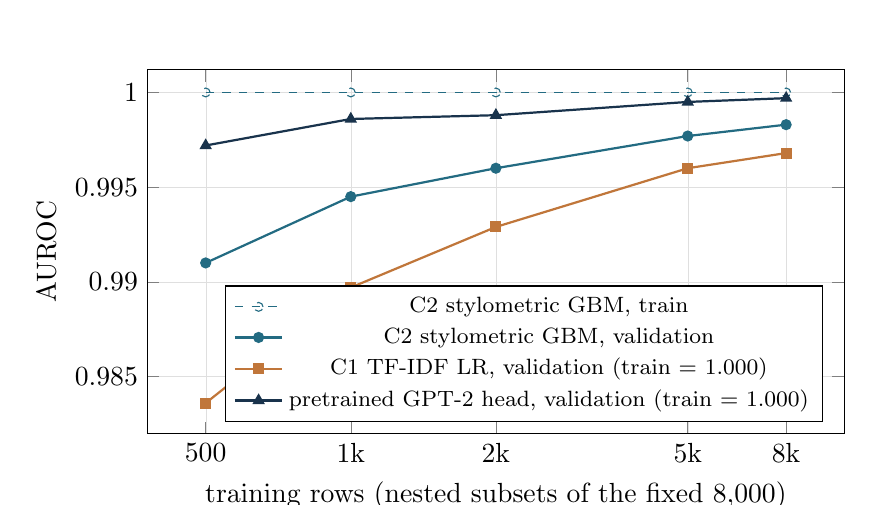
\begin{tikzpicture}
\begin{axis}[width=0.86\linewidth, height=6.2cm, xmode=log, log basis x=10,
  xtick={500,1000,2000,5000,8000}, xticklabels={500,1k,2k,5k,8k},
  xlabel={training rows (nested subsets of the fixed 8,000)}, ylabel={AUROC},
  ymin=0.982, ymax=1.0012, yticklabel style={/pgf/number format/fixed,/pgf/number format/precision=3},
  legend pos=south east, legend style={font=\footnotesize}, grid=both, grid style={line width=.1pt, draw=gray!25}]
\addplot[teal, dashed, mark=o, mark size=1.6pt] coordinates {
% <<gen curve:classical/results/experiments/learning_curve.csv:stylo_gbm:train_auroc
(500,1.0000) (1000,1.0000) (2000,1.0000) (5000,1.0000) (8000,1.0000)
% gen>>
};
\addlegendentry{C2 stylometric GBM, train}
\addplot[teal, thick, mark=*, mark size=1.6pt] coordinates {
% <<gen curve:classical/results/experiments/learning_curve.csv:stylo_gbm:val_auroc
(500,0.9910) (1000,0.9945) (2000,0.9960) (5000,0.9977) (8000,0.9983)
% gen>>
};
\addlegendentry{C2 stylometric GBM, validation}
\addplot[copper, thick, mark=square*, mark size=1.6pt] coordinates {
% <<gen curve:classical/results/experiments/learning_curve.csv:tfidf_lr:val_auroc
(500,0.9836) (1000,0.9897) (2000,0.9929) (5000,0.9960) (8000,0.9968)
% gen>>
};
\addlegendentry{C1 TF-IDF LR, validation (train = 1.000)}
\addplot[navy, thick, mark=triangle*, mark size=1.8pt] coordinates {
% <<gen curve:pretrained/results/learning_curve.csv:lm_gpt2:val_auroc
(500,0.9972) (1000,0.9986) (2000,0.9988) (5000,0.9995) (8000,0.9997)
% gen>>
};
\addlegendentry{pretrained GPT-2 head, validation (train = 1.000)}
\end{axis}
\end{tikzpicture}
\end{center}
\smallnote{Training AUROC is 1.000 at every size for all three models, so only C2's train curve is drawn.}
\question{Q2.3 [3 points].}{What does the curve suggest about overfitting, underfitting, and the value of more labeled examples?}
\textbf{No underfitting.} Every model separates its training rows perfectly (train AUROC 1.000) at every size, so training AUROC carries no information here; the validation curve is what matters.

\textbf{Overfitting shrinks with data but never disappears.} C2's train--validation gap falls from 0.009 at 500 rows to 0.0017 at 8,000. Each doubling adds about 0.002, and the curve is flattening. C1 starts lower (0.984) and gains about 0.003 per doubling, as expected for a model with close to a million sparse features. The pretrained GPT-2 head is at 0.997 with only 500 labels, because the LM supplies the representation.

\textbf{Value of more labels.} More labels \emph{of the same kind} would add little: at most a few thousandths, mainly for C1. The bigger gap is to test, whose domains and generators differ (C2 drops from 0.998 on validation to 0.960 on Kaggle). More \emph{diverse} labels, such as verse and new generators, would plausibly matter far more than more rows like these.

\section{Learning from unlabeled data (5 points)}
\textbf{Learning goal:} test whether the additional 3,000 unlabeled passages help.
\question{Q3.1 [2 points].}{Describe one method that uses \texttt{unlabeled.csv} (e.g., self-training, confidence-based pseudo-labeling, clustering, or feature learning). How did you prevent validation-label leakage?}
\textbf{Confidence-based self-training}, with hyperparameters held fixed:
\begin{enumerate}
\item Train on the 8,000 rows and score \texttt{unlabeled.csv}.
\item Label the 20\% highest-scored passages AI and the 20\% lowest human (1,200 pseudo-labels).
\item Retrain on the 8,000 rows plus these pseudo-labels.
\end{enumerate}
We ran 1 and 3 rounds (each round re-selects from the newest model) for C1, C2 and the pretrained GPT-2 head.

\textbf{Leakage control.} The validation rows are split off before anything is fit and scored once at the end. The pool is \texttt{unlabeled.csv} only (no test or validation text), and we checked that no unlabeled passage duplicates a validation passage (0 matches). The C3 tokenizer also uses \texttt{unlabeled.csv} text, never its labels (it has none).
\question{Q3.2 [2 points].}{Compare against a supervised baseline under the same held-out validation protocol.}
\begin{tabularx}{\linewidth}{@{}Yp{1.5in}@{}}\toprule Method & Validation AUROC \\ \midrule
% <<gen file:reports/tables/q32_semisup.tex
Supervised only (\texttt{lm\_gpt2}) & 0.99972 \\
Pseudo-labels, 1 round (\texttt{lm\_gpt2}) & 0.99972 \\
Pseudo-labels, 3 rounds (\texttt{lm\_gpt2}) & 0.99974 \\
\midrule
Supervised only (\texttt{tfidf\_lr}) & 0.99678 \\
Self-training, 1 round (\texttt{tfidf\_lr}) & 0.99675 \\
Self-training, 3 rounds (\texttt{tfidf\_lr}) & 0.99676 \\
Supervised only (\texttt{stylo\_gbm}) & 0.99831 \\
Self-training, 1 round (\texttt{stylo\_gbm}) & 0.99829 \\
Self-training, 3 rounds (\texttt{stylo\_gbm}) & 0.99835 \\
% gen>>
\bottomrule\end{tabularx}
\question{Q3.3 [1 point].}{Did it help? Give a concrete, evidence-based explanation (including possible noise in pseudo-labels).}
\textbf{No.} Every change is within $\pm$0.0001, below what 2,000 validation rows resolve.

\textbf{Why: the pseudo-labels carry no new information.} The passages confident enough to be selected are ones the model already gets right. For C2, every selected passage scored at least 0.99996 (AI) or at most 0.0001 (human); for the GPT-2 head, at least 0.9995 or at most 0.0005. Any wrong pseudo-labels are reinforced rather than corrected. The problem is uninformative pseudo-labels, not noisy ones.

\textbf{The pool also does not cover the shift.} \texttt{unlabeled.csv} has 1.2\% verse-like passages, like train (1.6\%), while test has 16.6\%. So it cannot teach what test needs.

\newpage
\section{Generalization and error analysis (20 points)}
\textbf{Learning goal:} characterize how well the selected model generalizes and where it fails. Use \textbf{labeled validation data}; hidden test labels and hidden domain/generator information are unavailable.

\question{Q4.1 [5 points].}{Compare training and validation AUROC for your final selected model. Is there a gap? What explanations are plausible?}
\textbf{Blend A:} training AUROC 1.00000 (0.999997), validation 0.99990, a gap of only 0.0001. At a 0.5 threshold it misclassifies 9 of 2,000 validation passages (3 false positives, 6 false negatives). The gap is small because most of the representation comes from pretrained LMs that never saw our labels, and validation is drawn from the same distribution as training. For comparison, the from-scratch C2 has a gap of 0.0017 (1.00000 against 0.99831), ordinary overfitting of 800 boosted trees.

\textbf{The gap that matters is to test:} 0.99990 on validation against 0.99161 public. Test has unseen generators and far more verse (16.6\% against 1.6\% of train), which validation cannot show. The shift hurts from-scratch models more: C2 falls from 0.99831 to 0.95995, and C3 from 0.98903 to 0.91502.

\question{Q4.2 [5 points].}{Evaluate performance over at least three text-length bins (define the bins), or another observable subgroup available in your data. Explain why you chose the grouping.}
\begin{tabularx}{\linewidth}{@{}Yrr@{}}\toprule Subgroup / bin (blend A, final model) & Count & Validation AUROC \\ \midrule
% <<gen file:pretrained/reports/tables/q42_subgroups.tex
$<$150 words (word count; 234 AI) & 380 & 1.00000 \\
150-250 words (word count; 444 AI) & 1049 & 0.99986 \\
$>$250 words (word count; 322 AI) & 571 & 0.99999 \\
prose (line structure; 804 AI) & 1400 & 0.99983 \\
short lines (lists, recipes) (line structure; 192 AI) & 575 & 1.00000 \\
verse (line structure; 4 AI) & 25 & 1.00000 \\
% gen>>
\midrule
\multicolumn{3}{@{}l}{\textit{C2 (from-scratch stylometric GBM), same rows}} \\
% <<gen file:classical/reports/tables/q42_subgroups.tex
$<$150 words (word count; 234 AI) & 380 & 0.99927 \\
150-250 words (word count; 444 AI) & 1049 & 0.99916 \\
$>$250 words (word count; 322 AI) & 571 & 0.99674 \\
prose (line structure; 804 AI) & 1400 & 0.99845 \\
short lines (lists, recipes) (line structure; 192 AI) & 575 & 0.99740 \\
verse (line structure; 4 AI) & 25 & 1.00000 \\
% gen>>
\bottomrule\end{tabularx}

\textbf{Groupings.}
\begin{itemize}
\item Word-count bins ($<$150, 150--250, $>$250 words): per-word rates and averaged LM statistics are noisier for short passages.
\item Line structure: verse ($\ge$4 lines, median $\le$10 words per line, no digits), short-line lists or recipes, and prose. Test is 16.6\% verse, and layout drives our stylometric model.
\end{itemize}

\textbf{Observed.} Blend A is at or above 0.9998 in every group. C2 is weakest on long passages (0.9967) and short-line lists (0.9974). Verse scores perfectly, but on only 25 rows (4 AI), so it is not informative. That is itself a finding: the subgroup that matters most for test is almost absent from the labelled data.

\question{Q4.3 [5 points].}{Analyze at least \textbf{five false positives and five false negatives} from your held-out validation set. Provide example IDs, predicted probabilities, and short failure hypotheses. Do not paste full passages unless essential.}
{\small\begin{tabularx}{\linewidth}{@{}p{0.45in}p{0.82in}p{0.42in}Y@{}}\toprule ID & Error type & P(AI) & Possible reason \\ \midrule
% <<gen file:pretrained/reports/tables/q43_errors.tex
\mbox{2696} & FP & 0.583 & Run-on, repetitive predictive-text-style ramble with no punctuation; DeBERTa and the GPT-2 token-stats-only model rank it 0.87-0.93 - repetitive low-perplexity text looks like small-model AI output. \\
\mbox{6479} & FP & 0.505 & Wire-style football news report with quotes (Solskjaer injury); every member sits near 0.5 - formulaic news prose is predictable to an LM. \\
\mbox{7384} & FP & 0.505 & Short, informal movie review with run-on sentences; members split around 0.5 - hypothesis: generic review phrasing is low-surprise for the LMs. \\
\mbox{9388} & FP (near miss) & 0.495 & Near miss (P=0.495, below 0.5): Wikipedia bio of composer Bright Sheng with a long list of orchestras; list-like encyclopedic prose is predictable. \\
\mbox{6138} & FP (near miss) & 0.489 & Near miss (P=0.489): Wikipedia article on a paramilitary group; formal encyclopedic register, like 9388. \\
\mbox{6331} & FN & 0.476 & AI bread recipe with ingredient lines and self-correcting notes ('it was my error to add...'); the token-stats-only model ranks it 0.17 - hypothesis: messy, human-like asides and recipe layout. \\
\mbox{2914} & FN & 0.487 & AI physics proposal with hard line wraps and two-space indentation like an arXiv abstract; DeBERTa ranks it 0.05 - hypothesis: copies human arXiv formatting and dense jargon (high perplexity). \\
\mbox{3938} & FN & 0.494 & AI wiki-style article (View Askew universe) with long lists of film titles; all members near 0.5 - proper-noun lists look human to token statistics. \\
\mbox{7049} & FN & 0.494 & AI spelt-dough recipe with bullet glyphs and scraped-web layout (also a stylo\_gbm FN); formatting mimics human scraped text. \\
\mbox{1602} & FN & 0.496 & AI wiki-bio with a hatnote and [1] citation markers (also a stylo\_gbm FN); copies Wikipedia scraping artefacts that train associates with human text. \\
% gen>>
\bottomrule\end{tabularx}}
\smallnote{Blend A, threshold 0.5. A false positive is human text predicted AI; a false negative is AI text predicted human. Blend A makes only 3 false positives at 0.5, so the two highest-scored humans below 0.5 are added as near misses. P(AI) is the blend's weighted mean member percentile.}

\question{Q4.4 [5 points].}{What recurring failure patterns did you identify, and how might you address one of them? Distinguish observed patterns from speculation.}
\textit{Observed.}
\begin{enumerate}
\item \textbf{Blend A's errors are disagreements, not confident mistakes.} Every error scores between 0.48 and 0.58. On 2696 and 2914, DeBERTa gives 0.87 and 0.05 while the LM-statistics members sit at 0.52--0.56.
\item \textbf{False negatives copy scraped-web layout.} Four of five are AI passages formatted like scraped web text: recipe ingredient lines, a Wikipedia hatnote with \texttt{[1]} markers, hard line wraps, bullet glyphs. Two of them (1602, 7049) are also confident errors of C2.
\item \textbf{False positives are formal, predictable human prose:} news, encyclopedia entries, generic reviews.
\end{enumerate}
\textit{Speculation.} The human training text was scraped, so its formatting artefacts became ``human'' cues that AI text in the same format exploits. Predictable human prose has the low perplexity that LM features associate with AI.

\textit{A fix to test.} Augment AI training passages with scraped-web formatting (citation markers, hard wraps, bullets), so formatting stops implying ``human''. Then measure the shared false negatives and the proxy. A related shortcut, line length, is the one we did fix (Q5).

\newpage
\section{Open-ended improvements and insights (15 points)}
\textbf{Learning goal:} propose and test one improvement beyond the required baseline comparisons. This can be simple: a targeted feature change, alternate regularization scheme, ensemble, different representation, augmentation, or training approach. Sophistication alone does not earn credit.

\question{Q5.1 [3 points].}{What specific question or hypothesis motivated your improvement? What weakness or opportunity did you observe?}
\textbf{Weakness.} Validation was saturated: every reasonable model scored 0.99 or more, the top dozen within 0.0005. Yet our first from-scratch uploads fell sharply on Kaggle: C1 0.963 $\to$ 0.886 and C3 0.985 $\to$ 0.832. Test differs from train: it has unseen generators and 16.6\% verse against 1.6\%.

\textbf{Hypothesis.} A held-out set that imitates this shift will (1) reveal \emph{why} models fail and (2) rank designs the way the leaderboard does. Changing the representation to remove the shortcuts it reveals, namely topic words for C1 and line length for C3, will raise Kaggle AUROC without tuning on Kaggle. The same proxy also chooses the blend weights for blend A.

\question{Q5.2 [4 points].}{What exactly did you change? Describe the baseline, the new approach and what you held fixed for a fair comparison.}
\textbf{The proxy} (evaluation only, never trained on) contains:
\begin{itemize}
\item 542 AI rewrites of training human passages and 816 AI poems and stories, written locally by seven open models never used in training (Appendix A);
\item 681 human poems and stories from held-out Project Gutenberg books \cite{gutenberg}.
\end{itemize}
These are pooled with validation scores into one AUROC, weighted so that 41\% is creative writing, like test. For the classical models, only rewrites of \emph{validation} passages are used, so no model has trained on a rewrite's source.

\textbf{Baselines.} C1 v1 (word 1--2 + in-word character 2--5 TF-IDF); C3 v1 (raw text); blend B (equal weights).

\textbf{Changes.}
\begin{itemize}
\item C1 v2 adds raw-text character n-grams and distorted-text word n-grams \cite{stamatatos2017}.
\item C3 v2 joins single line breaks and reads distorted text.
\item Blend A's weights come from greedy selection \cite{caruana2004} on the proxy.
\end{itemize}

\textbf{Held fixed.} Training rows, validation split, architectures, CDF blending rule, and hyperparameter selection by inner CV only. Each new version was uploaded once.

\question{Q5.3 [4 points].}{What were the measured results?}
{\small\begin{tabularx}{\linewidth}{@{}YrrY@{}}\toprule Configuration & Val. AUROC & Runtime & Relevant difference \\ \midrule
% <<gen file:pretrained/reports/tables/q53_improvement.tex
Baseline: blend B (equal weights, no eval-set tuning) & 0.99985 & 16 s & proxy 0.9906; unseen-generator 0.9958; Kaggle public 0.98848 \\
Improvement: blend A (greedy weights on the OOD proxy) & 0.99990 & 53.6 min & proxy 0.9928; unseen-generator 0.9970; Kaggle public 0.99161 \\
% gen>>
\midrule
% <<gen file:classical/reports/tables/q53_versions.tex
Baseline: C1 v1 (word + in-word char TF-IDF) & 0.96256 & 16 s & proxy 0.8708; Kaggle public 0.88583 \\
Improvement: C1 v2 (+ raw char, distorted n-grams) & 0.99678 & 23 s & proxy 0.9555; Kaggle public 0.96374 \\
Baseline: C3 v1 (raw text) & 0.98500 & 38 s & proxy 0.7699; Kaggle public 0.83201 \\
Improvement: C3 v2 (lines joined, distorted) & 0.98903 & 32 s & proxy 0.9258; Kaggle public 0.91502 \\
% gen>>
\bottomrule\end{tabularx}}

\textbf{Where the gains came from} (each model fit on the 8,000 rows; AUROC except ``verse FPR''):

{\small\begin{tabularx}{\linewidth}{@{}Yrrrrrr@{}}\toprule Model & Val. & Unseen gen. & Creative & Verse FPR & Proxy & Public \\ \midrule
% <<gen file:classical/reports/tables/q53_ood.tex
C1 v1: word + char\_wb TF-IDF & 0.9626 & 0.8728 & 0.7801 & 0.07 & 0.8708 & 0.88583 \\
C1 v2: + raw char, distorted word n-grams & 0.9968 & 0.9538 & 0.9237 & 0.31 & 0.9555 & 0.96374 \\
C3 v1: raw text & 0.9817 & 0.8791 & 0.6105 & 0.71 & 0.7699 & 0.83201 \\
C3 v2: lines joined, text distorted & 0.9881 & 0.8694 & 0.9329 & 0.24 & 0.9258 & 0.91502 \\
C2 (unchanged, reference) & 0.9983 & 0.9665 & 0.9343 & 0.78 & 0.9650 & 0.95995 \\
% gen>>
\bottomrule\end{tabularx}}
\smallnote{Verse FPR = share of held-out Gutenberg human poems/stories scored above the threshold that flags 5\% of validation humans. ``Public'' is the Kaggle file refit on 10,000 rows. Source: \texttt{classical/results/ood\_eval.csv}, \texttt{submission\_log.csv}.}

\question{Q5.4 [4 points].}{What did you learn? Did the results support the hypothesis? What limits the conclusion, and what would you try next?}
\textbf{Supported.} The proxy ranked the three first classical models exactly as Kaggle did: C2 0.965, C1 0.871, C3 0.770, against public 0.960, 0.886, 0.832. It also exposed the causes:
\begin{itemize}
\item \textbf{C3 learned ``short lines = AI''.} In train, human passages have long lines and AI passages short ones, so C3 flagged 71\% of human verse. Joining single lines cut this to 24\% and raised creative AUROC from 0.61 to 0.93.
\item \textbf{C1 relied on topic.} The topic-free views raised its unseen-generator AUROC from 0.87 to 0.95.
\end{itemize}
Kaggle confirmed both fixes from one upload each: C1 0.886 $\to$ 0.964, C3 0.832 $\to$ 0.915, each within about 0.01 of its proxy score. For the blends, the proxy put A first while CV could not separate them, and Kaggle agreed (0.99161 against 0.98848).

\textbf{Lesson.} Formatting is usually real signal (debiasing hurt the stylometric proxy, 0.974 $\to$ 0.915), but a model with no hand-made features can latch onto a single cue, and that shortcut must be removed.

\textbf{Limits.} The proxy's generators and archaic Gutenberg text are a guess at test. It has only 112 classical unseen-generator rows, and we chose designs after seeing it, so it is somewhat optimistic (C3 came in 0.011 below). The v1 leaderboard scores told us \emph{which} models to investigate.

\textbf{Next.} Test the scraped-web augmentation (Q4.4), and pretrain C3 self-supervised from scratch on train plus unlabeled text: it is still weakest on unseen generators (0.87).

\section{Code submission, reproducibility and AI assistance (10 points)}
\textbf{Submission format:} Submit a \textbf{GitHub PR URL} against the course repository. We will inspect the final code and its development history, not just the final snapshot. Do not squash away meaningful intermediate commits before review. Template \href{https://github.com/sekhari/human-or-ai-submissions}{here}.

\question{Q6.1 [5 points].}{Provide the PR URL, the entrypoint for training/evaluation, and the command used to generate \texttt{submission.csv}. State dependencies and random seeds.}
\textbf{PR:} [TODO: PR URL]. \textbf{Code:} \texttt{submissions/group-number-31/}. Its \texttt{README.md} covers setup and every command, and \texttt{MODELS.md} gives each submitted model's full pipeline.

\textbf{Entry points}, run from that folder:
\begin{itemize}
\item \texttt{train.py}: train on the 8,000 rows and score the fixed 2,000, or \texttt{--final} to refit on 10,000 and write the Kaggle file.
\item \texttt{predict.py}: writes \texttt{submission.csv}.
\end{itemize}
{\footnotesize\begin{verbatim}
python common/make_split.py              # re-create + check the validation split
python predict.py --model blend_a --committed --out submission.csv
                                         # final file, exactly as uploaded
python predict.py --model blend_a --out submission.csv
                                         # re-predict from the saved runs (GPU)
python train.py --model tfidf_lr         # C1: inner-CV search, fit 8k, score 2k
python train.py --model tfidf_lr --final # refit on 10k -> Kaggle file
python predict.py --model tfidf_lr --out submission.csv
\end{verbatim}}
\textbf{Environment.} Python 3.12; \texttt{pip install -r requirements.txt} (numpy, pandas, scikit-learn, LightGBM, tokenizers, PyTorch, Hugging Face Transformers). The classical track runs on a laptop CPU. The pretrained track needs a 12 GB GPU and, for an RTX 50-series card, PyTorch built with CUDA 12.8+. Kaggle CSVs are not committed; pass \texttt{--data-dir} or set \texttt{HOA\_DATA\_DIR}.

\textbf{Seeds.} 20261023 for the split, all CV folds and every fixed-split experiment; the 5-fold runs behind the pretrained uploads used seed 42.

\textbf{Reproduction.} \texttt{predict.py} reproduces the committed classical files exactly (maximum difference 0). Blend A rebuilt from the saved models matches the upload with Spearman 1.000000.

\question{Q6.2 [3 points].}{Give two or three examples of changes you made during development. Link to relevant commits or PR discussion and briefly explain what the experiments taught you.}
\begin{itemize}
\item \commit{fb3df12d56cf3f45b3d7664818888d9128c4523d}{fb3df12}, \commit{efb72f048cb76989e9d33f94779eb7106bfc4196}{efb72f0}, \commit{6316699fb7a326deb625b7bc0776a3a87533e1b3}{6316699}, \commit{dc302d22e1432fce759bd2a2851ae09dfd5fce0e}{dc302d2}: after C1 and C3 fell on Kaggle, we scored them on held-out shifted text. That found the topic and line-length shortcuts, and the rebuilt models went from 0.886 to 0.964 and from 0.832 to 0.915. \emph{Lesson:} when validation and the leaderboard disagree, build a test-like held-out set instead of tuning on the leaderboard.
\item \commit{1fc181fef044ef79830a9a0db09f32bc305f38e0}{1fc181f} $\to$ \commit{ed4ad2daeabbb6f05fc791791dff0edf34ced42e}{ed4ad2d} $\to$ \commit{77663a46bfcbc667df49d3aeb81d00485319b2f8}{77663a4}: a 35-job benchmark saturated CV (0.990--0.999), so we built the out-of-distribution proxy. The blend chosen on it won on Kaggle. \emph{Lesson:} saturated CV cannot choose between strong models.
\item \commit{6fb8406709d375571d760b4d23b11a131c61c44e}{6fb8406}, \commit{3754f3b7f2d07855ff6e01a9ef753e7f575d4698}{3754f3b}: removing C2's layout features cost 0.011 AUROC, and debiasing hurt the pretrained models too. \emph{Lesson:} formatting is real signal, so we kept it everywhere except the one model it misled.
\end{itemize}

\question{Q6.3 [2 points].}{How did you use AI tools (such as Claude, ChatGPT or Copilot) for code, debugging, analysis or writing? What did you verify or modify yourself?}
\textbf{Our decisions.} We decided the overall structure (two tracks on one fixed validation split), the model architectures, the candidate models and which analyses to run.

\textbf{Claude Code's role.} Claude Code (Anthropic) mainly wrote the code to those specifications and executed the experiments on our machines. It also helped draft report text, which we edited.

\textbf{What we verified and changed.}
\begin{itemize}
\item We read the data ourselves (verse, recipes, scraped-web layout, blank-line habits) and changed the pipelines along the way to match what we saw.
\item We checked every local score against the Kaggle score. When they disagreed (C1 and C3), we had the cause investigated and changed the models accordingly.
\item We made every Kaggle upload and checked that every number in this report comes from committed results files.
\end{itemize}

\textbf{Rules followed, specifically.}
\begin{itemize}
\item \textbf{Supervised labels come only from \texttt{train.csv}.} Every model, in both tracks, is fit on \texttt{train.csv} rows: 8,000 for validation experiments, all 10,000 for the Kaggle files. \texttt{unlabeled.csv} is used without labels, for C3's tokenizer and the self-training experiment (Q3), where pseudo-labels come from our own model.
\item \textbf{The proxy is held-out evaluation text, not training data.} The proxy is 1,358 AI passages we generated locally with seven open models plus 681 human passages from held-out Project Gutenberg books. No model was ever fit on it: all 72 logged pretrained runs list no external training files, and the classical models load only the competition CSVs.
\item \textbf{We used the proxy for model selection.} It chose blend A's seven weights over existing, already-trained models (Q5.2), and it decided between the v1 and v2 representations of C1 and C3. It never chose a hyperparameter; those come from 5-fold CV inside the 8,000 training rows. We report this selection, and the optimism it adds, in Q5.4.
\item \textbf{No outside model touched the test set.} The seven generators ran locally and only wrote new text; none labelled, scored or saw a test or validation passage. No external LLM API was used anywhere. Test passages were scored only by our own submitted models.
\item \textbf{No hidden labels.} We did not search for or use test labels, generator names or domain information from any source. The only feedback from Kaggle was the public score of each upload. We made 8 uploads (Appendix B), and each new version was uploaded once, not tuned against the leaderboard.
\item \textbf{Validation was not used for tuning.} The 2,000 validation rows are in no CV fold and were used only to report the chosen settings.
\item \textbf{All pretrained weights are disclosed} in Appendix A, including the generators and the models we tried but did not submit. The from-scratch models (C1--C3) use no pretrained weights.
\end{itemize}

\textbf{AI policy.} You may use AI assistants for coding, debugging, explanations, brainstorming, and editing. We expect each team to exercise its own judgment, run experiments, check outputs, and understand its submitted approach. Sending the entire assignment to an AI tool and submitting its unverified output without meaningful involvement does not satisfy the objectives of this project. We will use the PR history, reproducible experiments and report together as evidence of engagement. \emph{Commit counts and the presence of AI-generated code are not themselves grading criteria.} Do not fabricate results or retrieve hidden test labels.


\section*{Final submission checklist}
\begin{itemize}[label=$\square$]
\item Final probabilities submitted to Kaggle for every \texttt{test.csv} ID.
\item Completed report, with all required answers, tables, figures and sources, submitted as PDF.
\item GitHub PR linked on the report title page and in the course submission portal.
\item Code and dependencies recreate final predictions (within reasonable numerical tolerance).
\item Relevant experiments and seed/configuration details are recorded.
\item AI-use disclosure is complete; hidden labels were not retrieved externally.
\end{itemize}

\appendix
\section*{Appendix A. Pretrained models in the submitted blends}
All checkpoints come from the Hugging Face Hub. The from-scratch models (C1--C3, files D--F) use no pretrained weights.

{\small\begin{longtable}{@{}p{2.2in}rp{2.35in}p{0.8in}@{}}
\caption{The pretrained checkpoints inside blends A--C, and how each is used.}\label{tab:pretrained}\\
\toprule Checkpoint (Hugging Face) & Params & How we used it & In blends \\ \midrule\endfirsthead
\toprule Checkpoint (Hugging Face) & Params & How we used it & In blends \\ \midrule\endhead
\multicolumn{4}{@{}l}{\textit{Frozen language models: token statistics as features for a LightGBM head (weights never updated)}} \\
\hf{openai-community/gpt2} \cite{gpt2} & 124M & per-token log-prob, rank, entropy (15 stats) & A, B, C \\
\hf{openai-community/gpt2-medium} \cite{gpt2} & 355M & same statistics, larger LM & A, B, C \\
\hf{Qwen/Qwen2.5-0.5B} + \hf{-Instruct} \cite{qwen25} & 0.5B & Binoculars observer/performer pair \cite{binoculars}: perplexity, cross-perplexity, Binoculars score & A, B, C \\
\hf{Qwen/Qwen2.5-1.5B} + \hf{-Instruct} \cite{qwen25} & 1.5B & same, larger pair & A, B, C \\
\midrule
\multicolumn{4}{@{}l}{\textit{Encoders fine-tuned end to end as classifiers (5-fold; test score = mean of the fold models)}} \\
\hf{FacebookAI/roberta-base} \cite{roberta} & 125M & fine-tuned classifier & A, C \\
\hf{microsoft/deberta-v3-large} \cite{debertav3} & 435M & fine-tuned classifier & A \\
\hf{openai-community/roberta-large-openai-detector} \cite{solaiman2019} & 355M & GPT-2 output detector, fine-tuned further & A \\
\bottomrule
\end{longtable}}

\textbf{Used for evaluation only, not in any submitted model.} The out-of-distribution proxy (Q5) contains AI text that we generated locally with seven open models: Llama-3.2-3B-Instruct \cite{llama3}, Qwen3-4B-Instruct-2507 \cite{qwen3}, Phi-3.5-mini-instruct \cite{phi3}, SmolLM2-1.7B-Instruct \cite{smollm2}, Granite-3.1-2B-Instruct \cite{granite}, OLMo-2-1B-Instruct \cite{olmo2} and Pythia-1.4B \cite{pythia}. That text was scored, never trained on.

\textbf{Tried during development, not submitted.} DeBERTa-v3-base/small \cite{debertav3}, DistilRoBERTa \cite{distilbert}, ModernBERT-base \cite{modernbert}, ELECTRA-base \cite{electra}, the RoBERTa-base GPT-2-output detector \cite{solaiman2019}, and BGE \cite{bge} and E5 \cite{e5} sentence embeddings.

\section*{Appendix B. Kaggle submissions}
Every file we uploaded, in upload order. E and F were first uploaded as v1 and then replaced by v2 under the same letter (Q5). Validation = the fixed 2,000 rows. The full testing history of every model we validated, including those never uploaded, is in \texttt{SUBMISSIONS.md} in the repository.

{\small\begin{tabularx}{\linewidth}{@{}lYrrrl@{}}\toprule
File & Model & Val. AUROC & Public & Private & Commit \\ \midrule
% <<gen file:reports/tables/kaggle_uploads.tex
A & Blend A (final): 7 models, proxy-chosen weights & 0.99990 & 0.99161 & -- & \href{https://github.com/ZhenmanShen/human-or-ai-submissions/commit/c7c1e3e5c379f092b31d1ef745dbf2900d052f03}{\texttt{c7c1e3e}} \\
B & Blend B: 4 frozen-LM heads, equal weights & 0.99985 & 0.98848 & -- & \href{https://github.com/ZhenmanShen/human-or-ai-submissions/commit/c7c1e3e5c379f092b31d1ef745dbf2900d052f03}{\texttt{c7c1e3e}} \\
C & Blend C: blend B + RoBERTa-base & 0.99987 & 0.98845 & -- & \href{https://github.com/ZhenmanShen/human-or-ai-submissions/commit/c7c1e3e5c379f092b31d1ef745dbf2900d052f03}{\texttt{c7c1e3e}} \\
D & C2 stylometric GBM & 0.99831 & 0.95995 & -- & \href{https://github.com/ZhenmanShen/human-or-ai-submissions/commit/08cde9152812e9dc60a72a394012065253065643}{\texttt{08cde91}} \\
E (v1) & C1 TF-IDF + LR, first version & 0.96256 & 0.88583 & -- & \href{https://github.com/ZhenmanShen/human-or-ai-submissions/commit/d0cfc4c8c92c432b47f372ca6f7cf3db06f780c2}{\texttt{d0cfc4c}} \\
F (v1) & C3 Transformer, first version & 0.98500 & 0.83201 & -- & \href{https://github.com/ZhenmanShen/human-or-ai-submissions/commit/a0679175ad4b0fa0a04df438aad48b956f1b26f5}{\texttt{a067917}} \\
E & C1 TF-IDF + LR, v2 (raw char + distorted n-grams) & 0.99678 & 0.96374 & -- & \href{https://github.com/ZhenmanShen/human-or-ai-submissions/commit/05e04170434cf5204e08a0a844ad4e91aaf9045f}{\texttt{05e0417}} \\
F & C3 Transformer, v2 (lines joined, distorted) & 0.98903 & 0.91502 & -- & \href{https://github.com/ZhenmanShen/human-or-ai-submissions/commit/05e04170434cf5204e08a0a844ad4e91aaf9045f}{\texttt{05e0417}} \\
% gen>>
\bottomrule\end{tabularx}}

{\small
\begin{thebibliography}{99}\setlength{\itemsep}{1pt}
\bibitem{gpt2} A.~Radford, J.~Wu, R.~Child, D.~Luan, D.~Amodei, I.~Sutskever. Language Models are Unsupervised Multitask Learners. OpenAI technical report, 2019.
\bibitem{qwen25} Qwen Team. Qwen2.5 Technical Report. arXiv:2412.15115, 2024.
\bibitem{binoculars} A.~Hans et al. Spotting LLMs With Binoculars: Zero-Shot Detection of Machine-Generated Text. ICML 2024; arXiv:2401.12070.
\bibitem{roberta} Y.~Liu et al. RoBERTa: A Robustly Optimized BERT Pretraining Approach. arXiv:1907.11692, 2019.
\bibitem{debertav3} P.~He, J.~Gao, W.~Chen. DeBERTaV3: Improving DeBERTa using ELECTRA-Style Pre-Training with Gradient-Disentangled Embedding Sharing. ICLR 2023; arXiv:2111.09543.
\bibitem{solaiman2019} I.~Solaiman et al. Release Strategies and the Social Impacts of Language Models. arXiv:1908.09203, 2019 (the GPT-2 output detectors).
\bibitem{distilbert} V.~Sanh, L.~Debut, J.~Chaumond, T.~Wolf. DistilBERT, a distilled version of BERT: smaller, faster, cheaper and lighter. arXiv:1910.01108, 2019 (DistilRoBERTa follows the same recipe).
\bibitem{modernbert} B.~Warner et al. Smarter, Better, Faster, Longer: A Modern Bidirectional Encoder for Fast, Memory Efficient, and Long Context Finetuning and Inference (ModernBERT). arXiv:2412.13663, 2024.
\bibitem{electra} K.~Clark, M.-T.~Luong, Q.~V.~Le, C.~D.~Manning. ELECTRA: Pre-training Text Encoders as Discriminators Rather Than Generators. ICLR 2020.
\bibitem{bge} S.~Xiao et al. C-Pack: Packaged Resources To Advance General Chinese Embedding (BGE models). arXiv:2309.07597, 2023.
\bibitem{e5} L.~Wang et al. Text Embeddings by Weakly-Supervised Contrastive Pre-training (E5). arXiv:2212.03533, 2022.
\bibitem{hftransformers} T.~Wolf et al. Transformers: State-of-the-Art Natural Language Processing. EMNLP 2020 (System Demonstrations).
\bibitem{lightgbm} G.~Ke et al. LightGBM: A Highly Efficient Gradient Boosting Decision Tree. NeurIPS 2017.
\bibitem{sklearn} F.~Pedregosa et al. Scikit-learn: Machine Learning in Python. JMLR 12, 2011.
\bibitem{ma2023} Y.~Ma et al. AI vs.\ Human -- Differentiation Analysis of Scientific Content Generation. arXiv:2301.10416, 2023.
\bibitem{stamatatos2017} E.~Stamatatos. Authorship Attribution Using Text Distortion. EACL 2017.
\bibitem{bpe} R.~Sennrich, B.~Haddow, A.~Birch. Neural Machine Translation of Rare Words with Subword Units. ACL 2016.
\bibitem{transformer} A.~Vaswani et al. Attention Is All You Need. NeurIPS 2017.
\bibitem{caruana2004} R.~Caruana, A.~Niculescu-Mizil, G.~Crew, A.~Ksikes. Ensemble Selection from Libraries of Models. ICML 2004.
\bibitem{llama3} Llama Team, AI @ Meta. The Llama 3 Herd of Models. arXiv:2407.21783, 2024 (Llama 3.2 checkpoints).
\bibitem{qwen3} Qwen Team. Qwen3 Technical Report. arXiv:2505.09388, 2025.
\bibitem{phi3} M.~Abdin et al. Phi-3 Technical Report. arXiv:2404.14219, 2024 (Phi-3.5 checkpoints).
\bibitem{smollm2} L.~Ben Allal et al. SmolLM2: When Smol Goes Big. arXiv:2502.02737, 2025.
\bibitem{granite} IBM Granite Team. Granite 3.1 language models (model card, \texttt{ibm-granite/granite-3.1-2b-instruct}), 2024.
\bibitem{olmo2} Team OLMo. 2 OLMo 2 Furious. arXiv:2501.00656, 2025.
\bibitem{pythia} S.~Biderman et al. Pythia: A Suite for Analyzing Large Language Models Across Training and Scaling. ICML 2023.
\bibitem{gutenberg} Project Gutenberg. \url{https://www.gutenberg.org}.
\end{thebibliography}}

\end{document}
